
\chapter{Antecedentes}

En el capítulo 1 se habla a grandes rasgos de la estructura implícita de la modelación. Un sector importante es el del problema inverso. Aquí formalizaremos el concepto y detallaremos sus lineamientos. Se describe el enfoque bayesiano del problema inverso, que es un paradigma ampliamente estudiado. Otro enfoque al problema inverso es el operativo, el cual se aborde desde el problema directo como un operador actuando en el modelo, y el problema inverso como un operador inverso de este. Este último enfoque sale de los límites de estudio del texto. 

\section{Problema inverso}

El estudio del problema inverso se remonta a mediados del siglo 17. Los físicos contemporáneos interesados en la relación causa-efecto de diferentes fenómenos físicos lograron predecir el comportamiento en la dinámica subyacente. Así, para la ley de gravitacional de newton, una vez obtenidas las masas de los cuerpos celestes (causas) es posible predecir las trayectorias que siguen en el tiempo (efecto). Estudiar los efectos de un fenómeno dada ciertas causas es el problema directo, se requiere la metodología descrita en la introducción. El problema inverso toma la dirección opuesta, dados los efectos, es de interés investigar las causas que lo ocasionaron. Retomando un ejemplo newtoniano, dado un campo gravitatorio circundando cierto cuerpo celeste, es de interés conocer la masa de dicho cuerpo. El problema inverso padece de no ser único, suele ser el caso que a ciertos efectos se correspondas varias causas. el hecho de que no exista una mapeo uno a uno entre causa y efecto complica el problema inverso. Sin embargo, la información que se tenga a priori del fenómeno es crucial para determinar con una menor ambigüedad las causas. 

\subsection{Modelos descritos por ODEs}

Los modelos matemáticos para describir fenómenos pueden venir de una amplia variedad de modelos. Tomese que se desea describir los costos de la renta de inmuebles en cierta ciudad $Y$ (efecto). Supongase que de análisis previos se concluyo que dicho fenómeno esta vinculado al tamaño del inmueble $X_1$, número de habitaciones $X_2$, ingreso medio por habitante $X_3$ (causas). Un modelo plausible es por modelos lineales generalizados
\begin{align}
    Y = G(\beta_0 + \beta_1 X_1 + \beta_2 X_2 + \beta_3 X_3) + \varepsilon
    \label{2.1.1.01}
\end{align}
donde $G$ es la función liga, $\varepsilon \sim N(0,\sigma^2)$ un error aleatorio y $\beta = (\beta_0, \beta_1, \beta_2, \beta_3)$ son los parámetros del modelo. El problema directo considera predecir el valor de $Y$ conociendo $X = (X_1,X_2,X_3)$ y los parámetros del modelo $\beta$. Para esta clase de modelos el problema directo no representa complejidad. En contraste, el problema inverso precisa estimaciones de $\beta$  y $\sigma$ dada muestras de $Y$ y $X$, siendo un problema no trivial. 

% Introducir los modelos por EDOs
El análisis del problema inverso para modelos en general es bastante amplio. Por ello es necesario restringirlo a una clase menor de modelos, siendo estos los modelos dados por ODEs. Considerese un modelo para describir al dinámica de $y(t)$ a lo largo del tiempo $t$. Los modelos considerados son aquellos que se pueden expresar de la forma
\begin{align*}
    G(t,y(t),y'(t),y''(t),...) = 0
\end{align*}
que es una ODE con $G$ una función continua conocida.

Más aún, se puede obtener el análisis del problema inverso para sistemas de ecuaciones diferenciales ordinarias. Esto es
\begin{align*}
    \left\{
        \begin{matrix}
        G_1(t,y_1(t),y_1'(t),...,y_2(t),y_2'(t),..., y_d(t),y_d'(t),...)=0\\
        G_2(t,y_1(t),y_1'(t),...,y_2(t),y_2'(t),..., y_d(t),y_d'(t),...)=0\\
        \vdots
        \\ 
        G_d(t,y_1(t),y_1'(t),...,y_2(t),y_2'(t),..., y_d(t),y_d'(t),...)=0\\
       \end{matrix}
    \right.
\end{align*}
con $G_1, G_2, ..., G_d$ funciones continuas conocidas.

Observemos que la restricción implica restringir las variables en un soporte continuo, por lo que modelos como (\ref{2.1.1.01}) no se consideran para este análisis. En el capítulo 3 se detallan tres modelos de los cuales se consideraron los análisis del problema inverso. Dentro de estos se consideran modelos como la dinámica de caída libre sujeto a fricción, donde la distancia recorrida se describe por
\begin{align}
    mx''(t) = mg - bx'(t)
    \label{2.1.1.03}
\end{align}
con $m, g, b$ parámetros del modelo.

Dada las condiciones iniciales, los parámetros del modelo definen unívocamente el modelo por el teorema de unicidad de ecuaciones diferenciales. Consideremos el espacio de parámetros $\Theta$ que a su vez es la familia de \textit{submodelos} posibles descrito por la ODE. 


El problema directo es entonces aquel que dado un $\theta \in \Theta$ obtiene la trayectoria o solución de la ecuación diferencial. Dicho problema esta bien definido, pues resolver la ODE es posible al menos numéricamente. Denotemos por $\mathcal{Y}$ a las soluciones posibles de la ecuación diferencial. De esta forma existe un mapeo del espacio $\Theta$ a $\mathcal{Y}$ el cual llamaremos \textbf{Forward map}. El Forward map es 
\begin{align*}
    \theta \mapsto F(\theta) 
\end{align*}
donde $\theta \in \Theta$ y $F(\theta) \in \mathcal{Y}$.

Para el modelo dado en (\ref{2.1.1.03}) una vez dado $\theta = (m,g,b)$ la solución $x(t) \in \mathcal{Y}$ se obtiene del forward map, que en otras palabras es simplemente la solución analítica o numéricamente de la ecuación diferencial.

\section{Solución bayesiana a  problemas inversos}


Existen dos razones principalmente para que las observaciones de un modelo no concuerden exactamente con las predicciones dadas por el mismo. La primera se debe a errores de medición por la incertidumbre de los aparatos de medición. La segunda se befe a los defectos propios del modelo, pues a pesar de que el modelo pretende describir el fenómeno de interés este nunca es el mismo fenómeno, por lo que el concepto de modelo exacto no es concebible.


El paradigma bayesiano para problemas inversos toma una metodología establecida en cuantificar la incertidumbre en los parámetros del modelo. Su objetivo es establecer una medida de probabilidad posterior a las observaciones de la trayectoria del modelo. Equivalentemente, se busca la distribución $\pi(\theta|\mathbf{y})$ donde $\mathbf{y} = (y_1,...,y_n)$ son las observaciones de la trayectoria a lo largo del tiempo $t_1, t_2, \cdots, t_n$. Partiendo de una distribución inicial, conocida como distribución a priori, se establece una mediada de probabilidad $\pi(\theta)$ sobre los parámetros $\theta$ previo a las observaciones de la trayectoria con la información conocida del fenómeno y del modelo.

Como ya se ha mencionado, no se espera que las observaciones de la trayectoria coincidan con las predicciones del modelo. Para establecer la distribución de los errores necesitamos considerar el forward map a tiempos fijos $t_i$. En modelos dinámicos, aquellos que evolucionan en el tiempo, las predicción obtenidas se obtienen del forward map. Recordemos que fijando un vector de parámetros $\theta$ el forward map nos da la solución a la dinámica para el modelo, es decir $F(\theta) = y(t)$. Así en este caso, el forward map es una función en el tiempo. Para considerar las predicciones a cierto tiempo $t_i$ se toma solo $y(t_i)$. Usando la notación del forward map decimos que la predicción a tiempo $t_i$ es $F_{\theta}(t_i)$

De esta forma, se establece que las discordancias entre observaciones y predicciones siguen una distribución. Así se establece
\begin{align*}
    y_i = F_{\theta} (t_i) + \varepsilon_i, \:\:\:\:\:\: \varepsilon_i \sim N(0,\sigma^2)
\end{align*}

En consecuencia, se ha establecido una distribución para las observaciones $y_i$ las cuales tienen asociada una verosimilitud sobre $\theta$ y $\sigma$. Como se consideran errores independientes, pues se tratan de errores de medición, la verosimilitud se sigue de
\begin{align*}
    \mathcal{L}(\theta,\sigma) &= f(\mathbf{y}|\theta) = \prod_{i = 1}^{n} \frac{1}{\sqrt{2\pi \sigma^2}} \exp \left \{ -\frac{1}{2\sigma^2}\left(y_i - F_{\theta}(t_i)\right)^2 \right \} , 
\end{align*}
simplificando
\begin{align*}
    \mathcal{L}(\theta,\sigma) = \left(\frac{1}{2\pi \sigma^2}\right) ^{n/2}\exp \left \{  -\frac{1}{2\sigma^2}\sum_{i = 1}^{n} \left(y_i - F_{\theta}(t_i)\right)^2 \right \},
\end{align*}
Del teorema de Bayes, se sigue que la distribución posterior para los parámetros es
\begin{align}
    \pi(\theta| \mathbf{y})  = \frac{f(\mathbf{y}|\theta)\pi(\theta)}{\int f(\mathbf{y}|\theta)\pi(\theta)d \theta}
    \label{2.2.04}
\end{align}
la constante de integración $h(\mathbf{y}) = \int f(\mathbf{y}|\theta)\pi(\theta)d \theta$ es también la constante de normalización para la distribución posterior. 

Salvo en análisis conjugado, donde la distribución a priori y la distribución posterior pertenecen a la misma familia, la obtención analítica de la constante de normalización $h(\mathbf{y})$ es un problema complejo. De aquí surge la necesidad de métodos numéricos para determinar la distribución posterior con precisión. 

En el caso que $\Theta \subset \mathbb{R}$ utilizar métodos numéricos de integración para $h(\mathbf{y})$ es plausible, sin embargo para $\Theta \subset \mathbb{R}^d$ para $d>1$ los errores de calculo toman un rol no despreciable.

\section{Método MCMC}

Obtener la distribución posterior (\ref{2.2.04}) con el método de Markov Chain Monte Carlo (MCMC) evita la aproximación de calcular $h(\mathbf{y}$). En su lugar muestrea de la distribución posterior, obteniendo así estimaciones a la distribución y por ende estimaciones a cualquier momento de la misma. Los métodos MCMC busca encontrar una cadena de Markov cuya distribución estacionaria sea la distribución objetivo $f(x)$ sin necesidad de directamente simular de ella. 


\subsection{Algoritmo Metropolis-Hastings}

El algoritmo de Metropolis-Hastings es un método de MCMC para generar muestras de una distribución objetivo $f(x)$ partiendo de muestras de una distribución propuesta $q(y|x)$ que no son necesariamente simétricas. 

El algoritmo de Metropolis-Hastings genera una cadena $X_0, X_1, \cdots, X_N$. El algoritmo construye recursivamente la cadena dependiendo solamente del estado previo, es decir preservando la propiedad de Markov. El estado inicial $X_0$ se toma aleatoriamente. Luego, teniendo hasta el estado $X_i$, el estado $X_{i+1}$ se obtiene siguiendo 
\begin{enumerate}
    \item Generar una propuesta $Y \sim q(y|X_i)$.
    \item Calcular $\rho$ 
    \begin{align*}
        \rho = \min \left \{ \frac{f(y)q(x|y)}{f(x)q(y|x)}, 1  \right \} 
    \end{align*}
    \item Realizar un experimento Bernoulli con probabilidad de éxito $\rho$.
    \begin{align*}
        X_{i+1} = \left\{\begin{matrix}
            Y & \text{probabilidad} \rho  \\ 
            X_{i}& \text{probabilidad} 1- \rho  
           \end{matrix}\right.
    \end{align*}
\end{enumerate}

En el siguiente gráfico se muestra un diagrama de flujo del algoritmo Metropolis-Hastings.

\begin{figure}[H] 
    \centering 
    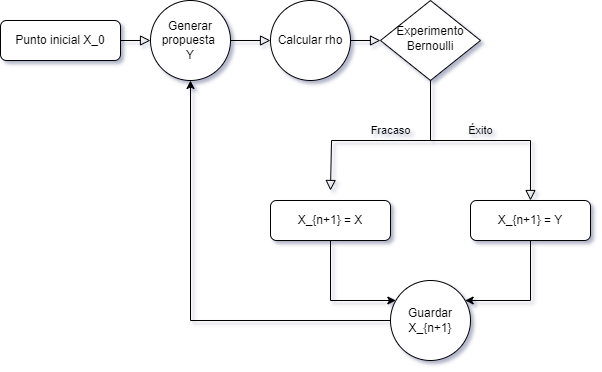
\includegraphics[width = 14 cm]{MCMC.png} 
    % \caption{}
    \label{Fig. }
\end{figure} 


\section{Forward map aproximado y consistencia}


La propuesta principal a la metodología ya establecida para abordar el problema inverso con el enfoque bayesiano es considerar aproximaciones del forward map. Existen diferentes maneras de hacer las aproximaciones del forward map. La forma propuesta es considerar una discretización del espacio de parámetros $\Theta$. Usando coordenadas, cada $\theta \in \Theta \subset \mathbb{R}^d$ se puede escribir como $\theta = (\theta_1, \theta_2, \cdots, \theta_d)$. Luego, considerese una partición equidistante $[\theta_i^{min},\theta_i^{max}]$ para todo $i \in \{1,\cdots,d\}$ donde $\theta_i^{min}$ y $\theta_i^{max}$ son cotas para el espacio de parámetros que contenga la masa de probabilidad, puede pensarse en tomar cuantiles de $0.01$ y $0.99$ respectivamente de la distribución marginal a priori para $\theta_i$. Consideremos que cada coordenada se particiona en $M$ puntos, luego hay $M^d$ puntos de la partición en el espacio de parámetros, denotando la malla como $\tilde{\Theta}\subset \Theta$.

Una vez establecido un enmallado de $\Theta$, se calcula el forward map solo para las intersecciones del enmallado. Así para cada $\tilde{\theta}_1, \tilde{\theta}_2, \cdots, \tilde{\theta}_{M^d}$ se obtiene el forward map $\tilde{y}_i = F(\tilde{\theta}_i)$ siendo cada una de estas funciones continuas. Posteriormente, para aproximar el Forward map en puntos $\theta \not\in \tilde{\Theta}$ se propone buscar a los $k$ puntos $\tilde{\theta}$ más cercanos en distancia euclideana. Denotando los $k$ vecinos de la malla más cercanos a $\theta$ por $\hat{\theta}_1, \cdots, \hat{\theta}_k$ cada uno a una distancia $d_1, \cdots, d_k$ de $\theta$. La aproximación al forward map es
\begin{align}
    F^{*}(\theta) = \sum_{i = 1}^{k} \frac{1}{d_i} \tilde{\theta}_i
\end{align}
que es una suma ponderada inversamente por las distancias, ya que se pretende que parámetros `lejanos' de $\theta$ tengan menor relevancia que los `cercanos'. 

% Esta estructura de aproximación se presta a la interpretación de que la información obtenida en mallas finas sea transmitidas a los vecinos.

% Convergencia

\section{Necesidad de trabajar con aproximaciones del Forward map}

Existe una ventaja operativa de trabajar el problema inverso con el forward map aproximado pues como veremos en el capítulo 3 los tiempos de ejecución son menores comparado con el forward map ordinario. 

